\section{Summary} \label{sec:summary}

\subsection{Applicability and Limitations}

It is important to remember that the range of physical conditions in
which Grackle can be considered valid is not unlimited.  In Figure
\ref{fig:valid_range}, we show the rough density range over which
different components of the solver is valid.  The high density limit
of the non-equilibrium solver is set roughly by the reactions present
in the network and the range over which their rate coefficents are
trusted.  The limits on the cooling tables correspond to the density
range over which they were calculated with.  Users are especially
cautioned against exceding the upper density limit of the tabulated
cooling solver.  The critical density above which energy levels are
populated according to LTE exceeds the upper limit of the tables for
many metal coolants \citep{2008MNRAS.385.1443S}.  Thus, these tables
do not capture the NLTE to LTE transition where the cooling rates
change from scaling as $\rho^{2}$ to $\rho$.  Hence, extrapolation
beyond the upper limit will result in vast overprediction of the
cooling rate.  If the use-case requires exceeding this limit, then the
high density metal table should be used in conjunction with the
non-equilibrium solver.  It is also extremely important to remember
that all Grackle calculations are based on the assumption that the
medium is optically thin.  In practice, the length scale of optical
thickness will become very short as density increases.

\begin{figure}
  \centering
  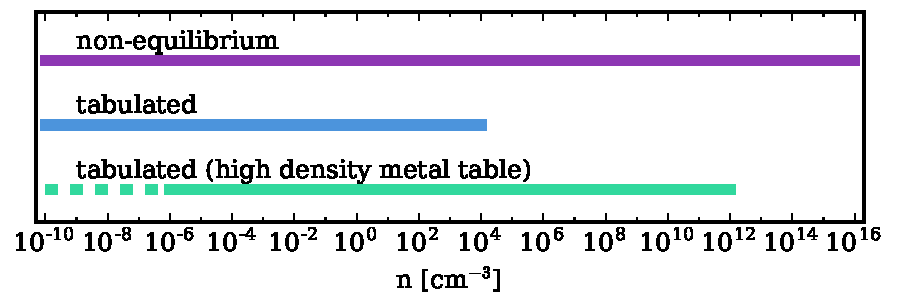
\includegraphics[width=0.48\textwidth]{valid_range.pdf}
  \caption{
    The appropriate density range for different versions of the
    Grackle solver.  The high density metal cooling table (bottom)
    explicitly spans the density range, 10$^{-6}$ cm $^{-3}$ $< n <$
    10$^{12}$ cm $^{-3}$, but extrapolation down to $n = 10^{-10}$ cm
    $^{-3}$ is still valid, as indicated by the dashed line.  For each
    of these, the valid temperature range is roughly 1 K to 10$^{9}$
    K.
  } \label{fig:valid-range}
\end{figure}

- Remind reader that cooling lengths are potentially very short and
having a fancy model is perhaps not very relevant at 1kpc
resolution. Can give some guidance of how to apply this.

\begin{figure*}
  \centering
  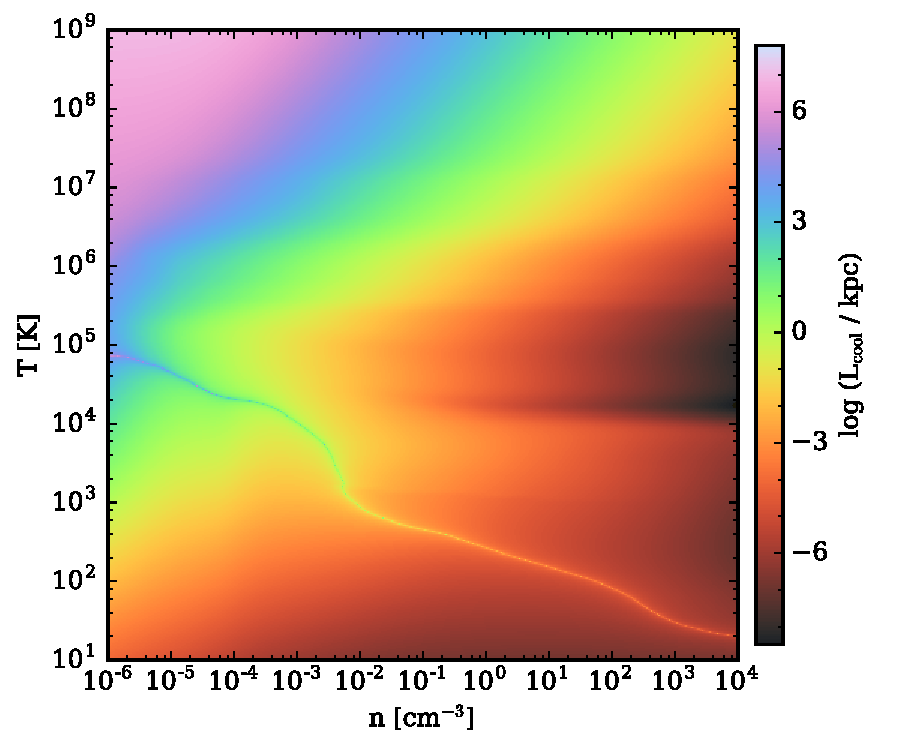
\includegraphics[width=0.84\textwidth]{cooling_length.pdf}
  \caption{
    The cooling length, defined as the product of the Jeans length and
    the cooling time, as a function of number density and temperature
    for a gas with solar metallicity exposed to a radiation field
    defined by the model of \citet{2012ApJ...746..125H} at z = 0.  The
    narrow line extending from the middle, left to the bottom, right
    represents the temperature where heating and cooling are
    balanced.  Above this line, the gas is being cooled while below
    the line it is being heated.
  } \label{fig:cooling-length}
\end{figure*}

\subsection{codes which have Grackle implementations}


\subsection{Future Directions} \label{Future_Directions}

\subsubsection{Including new rates and models in Grackle}
\jr{} The current code structure is highly integrated. This makes introducing new rates for the 
chemical network or cooling network a rather intricate task requiring multiple changes throughout the code. 
Apart from the fact that this is more time consuming it is also much more error prone. In a future release of the 
code the modularity of the code will be increased greatly. There will be a function to populate the species 
rate coefficients and a function to populate the cooling coefficients. Seperate template files can then be 
updated by a developer wishing to use their own rates. This file can then be included in the build and a flag
set to indicate the new rates be used in place of the old rates. Furthermore, a similar method will be 
implemented for solving the network. A template network solver will be available which the developer can use to 
implement a new network with a developer determined number of species. The developer will be responsible for
updating only three files to achieve a solution to their own chemical network. 

\subsubsection{Connection to Radiative Transfer}

\subsubsection{Multiple element cooling}

\subsubsection{Other heating sources?}
